\FloatBarrier
\subsection {Particle identification}

\FloatBarrier
\subsubsection{Time Projection Chamber (\TPC)}

Besides track reconstruction, \TPC\ also can measure ionization energy loss of the charged particles which can be used in particle identification.

\FloatBarrier
\subsubsection{Time of Flight (\TOF)}

\begin{figure}[ht]
    \begin{subfigure}{.49\textwidth}
        \centering
        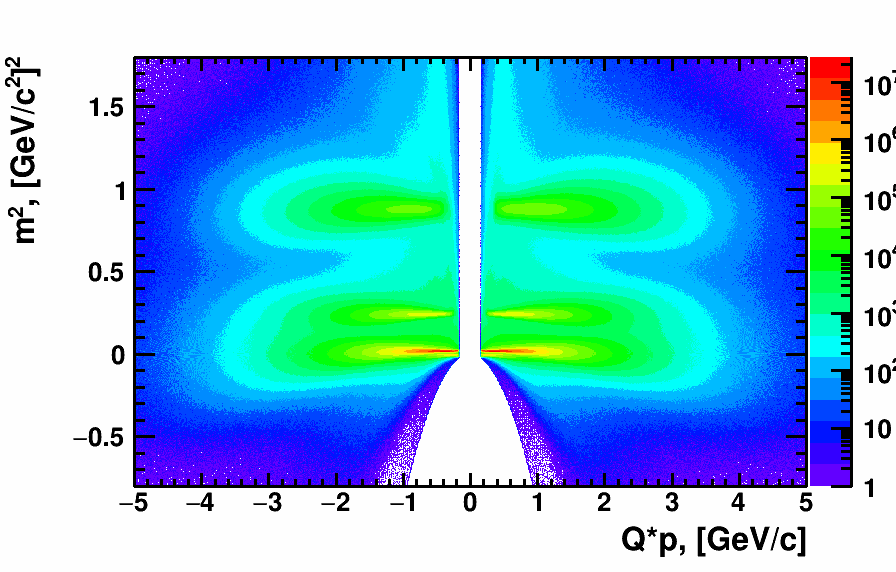
\includegraphics[width=1.\linewidth]{Figures/M2Qp_before_PID.png}
        %\caption{a}
    \end{subfigure}
    \begin{subfigure}{.49\textwidth}
        \centering
        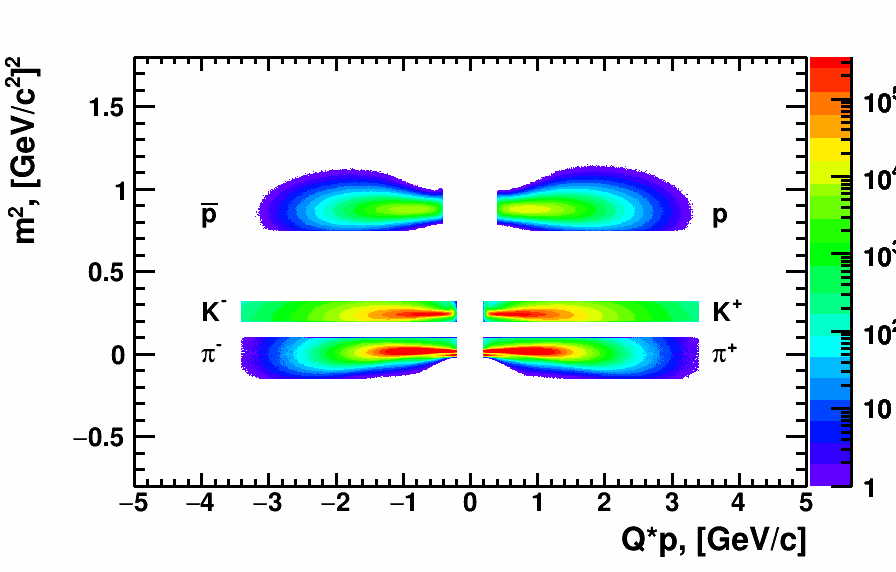
\includegraphics[width=1.\linewidth]{Figures/M2Qp_after_PID.png}
        %\caption{b}
    \end{subfigure}
    \label{fig:M2vsQp}
    \caption{$m^2$ estimated using \TPC\ and \TOF\ detectors vs charged total momentum $Q\cdot p$ before (left) and after (right) \PID\ procedure.}
\end{figure}